\documentclass[report.tex]{subfiles}

\begin{document}

\section*{Introduction}

Electronics sports, which will from now on be referred to as esports, are a form of competition using electronic systems, in particular video games, controlled by human players. In recent years the revenue and audience have seen a rapid growth with an estimation of over 300 million viewers in 2016 and over \$450 million in global revenue, and it is expected to see a formidable growth in the near future.\footnote{https://newzoo.com/insights/articles/esports-revenues-will-reach-696-million-in-2017/}

The esports industry utilizes many different platforms such as personal computers, x-box, playstation, and since everything is electronic we could potentially utilize all that data that is being generated for various kinds of analyses. That could help organizations/teams find better strategies, improve the viewer experience, and help newcomers getting accustomed the different games in a short time span.

\subsection*{DotA 2}

Defense of the Ancients (DotA 2) is a so called multiplayer online battle arena (MOBA) video game developed by Vale Corporation made first available in 2011. The game plays out as two teams of 5 player against each other where every player controls a hero, a character with unique abilities. The aim is to destroy the opponents ancient and thus win the game. The game is played in two phases, picks/bans and actual gameplay, and in this report the focus is on picks/bans that is very tactical because heroes have their strength and weaknesses. As of \today there are 114 unique heroes.

\subsubsection*{Picks/Bans}

The picks/bans phase is where the two teams pick their heroes that will be played during the gameplay phase. Each team has to pick 5 heroes, ban 5 heroes, and no team can pick banned heroes. To simplify the way this works, it starts out with both team banning 2 heroes each, then pick 2 heroes each, ban 2 heroes each, pick 2 heroes each, ban 1 hero each, and lastly pick 1 hero each.

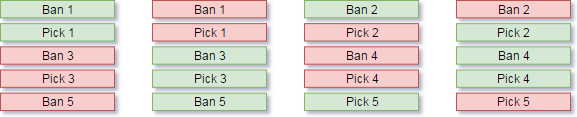
\includegraphics[width=\textwidth]{./images/dota2}

\end{document}
